\chapter{Fundamental Blocks of the Research} \label{chapter_two}


\section{Image Stabilisation}
If a camera is not stationary during video capture the output video quality may degrade and it may not look very good. Depending on the movements during capture, it may look very shaky or even the subjects of the video may not be properly visible. This is very undesirable and can cause visual discomfort \citep{jia2012probabilistic}. The solution to this maybe to keep the camera steady by mounting it on stable tripod or to a rigid object. But this is not practically possible all the time. There are various scenarios in which the camera may move around a lot and the movements may not be smooth at all e.g an action camera mounted on a helmet or a bicycle, a camera mounted on a car or a robot in wild or some move-able rig or robot arm.

The motion of the camera can be high-frequency tremors due to vibration, shaking or jiggling of the mounting point \citep{ryu2012robust} or low frequency such as movement of handheld camera during walking \citep{dis_review}. Practically, in most of the video recording scenarios, the camera will have some movement. The goal of image stabilization is to create a output video with same visual content without the undesired movements. 

% Start: Image Stabilisation
\subsection{Types of Image Stabilisation}
To deal with such movements and to make the video stable various techniques exist. These techniques are grouped in two categories:

\begin{itemize}
\item Hardware Image Stabilization
\item Digital Image Stabilization  
\end{itemize}
There are techniques which combine both these methods and are called Hybrid Image Stabilization techniques.

The goal of each of these stabilization techniques is to estimate the motion or pose and then do something to counteract that motion. I will talk about Pose-Estimation in depth in the later sections of this report. For now, let' see how these movements are countered or how the video is stabilized in each of these techniques.

\subsubsection{Hardware Image Stabilisation (HIS)}
Hardware image stabilization at its core means moving the lens or the image sensor or the camera setup itself to counteract these movements while recording the video in the first place. The movements of camera can be minimised by the use of mechanical stabilizers like tripods or dollies \citep{5995525}. The use of electronic gimbals for video recording has also increased recently for both professionals and hobbyists. Video can also be stabilised by varying the optical path between lens and the image sensor. This is generally achieved by using electronic motors and IMU sensors to move around the lens or the image sensor or both to cancel out the motions. After the motions have been counter-acted upon, images are captured which results in a stabilized video output as seen in figure \ref{fig:his}. These methods although mostly effective are not perfect and have both advantages and disadvantages.

\begin{figure}
\centering
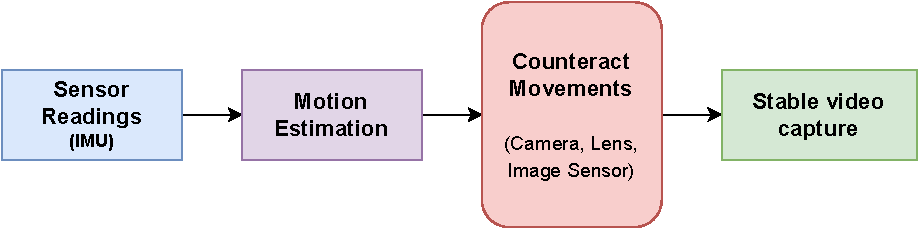
\includegraphics[scale=0.6]{images/fig_chapter2/2_1_his.pdf}
\caption{Hardware Image Stabilization}
\label{fig:his}
\end{figure}

\textbf{Advantages of HIS: }

\begin{itemize}
\item No post-processing for stabilization needed.
\item Works irrespective of the nature of object being captured.
\item Full image without cropping can be used.
\item Shutter Speed of the camera can be reduced
\end{itemize}

\textbf{Disadvantages of HIS:}
\begin{itemize}
\item Camera setups are very bulky.
\item These solutions can be very expensive.
\item More moving parts means higher maintenance.
\item Cannot be improved once hardware is implemented.
\item No possible on all camera setups.
\end{itemize}

\subsubsection{Digital Image Stabilisation (DIS)}
Digital Image Stabilization also called Digital Video Stabilization (DVS) is a software based image stabilization technique \citep{dis_review}. The technique here is similar what is done is HIS i.e. first motion of the camera is estimated (pose-estimation) and based on this, the image is stabilized. The difference here is that after pose estimation is done, instead of moving around the hardware a suitable transformation (warping) is applied to the image \citep{dis_feat_track} as shown is figure \ref{fig:dis}. The resulting stabilized image and hence the video is motionless irrespective of the camera motions. I will discuss this in more depth in the upcoming sections of this report. DIS can be a very powerful technique but like other methods and techniques, it has its advantages and disadvantages.

\begin{figure}
\centering
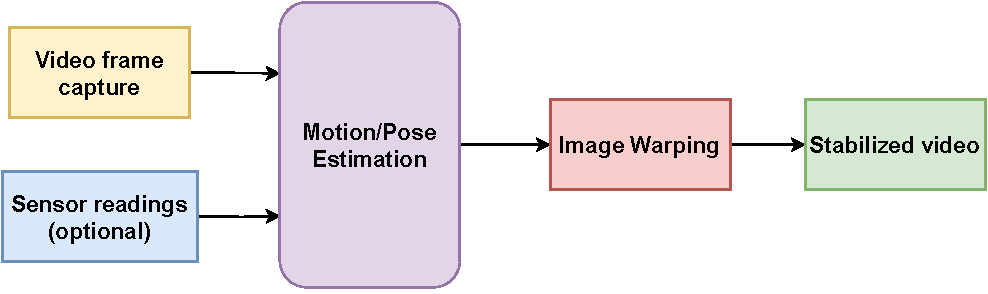
\includegraphics[scale=0.6]{images/fig_chapter2/2_1_dis.pdf}
\caption{Digital Image Stabilization}
\label{fig:dis}
\end{figure}

\textbf{Advantages of DIS: }
\begin{itemize}
\item Cost effective.
\item Smaller camera setups can be used.
\item No necessary changes need to be made to the camera setup for DIS.
\item Can be achieved using IMU sensors for pose estimation which are not very expensive.
\item Can be applied to any video; even the historic ones.
\item Different DIS algorithms can be used on a single video in post processing.
\item Relatively easy to modify DIS software.
\end{itemize}

\textbf{Disadvantages of DIS:}
\begin{itemize}
\item The resolution of the output images (video) is reduced (generally by 5 to 10 percent).
\item May require some manual labour (like in Adobe Premiere Pro: manual feature tracking).
\item Some videos are very difficult (even impossible) to stabilise if there is too much vibration or the features are not visible.
\item May require a lot of computational power (optical flow)
\end{itemize}
For my research purpose I will be using digital image stabilization.  I will be discussing in the future sections why I am choosing this technique. First, there are some other topics I need to discuss.

% Start: Pose Estimation
\section{Camera Motion Estimation for Image Stabilization}
Camera motion (pose) estimation is very important and one of the most challenging part of image stabilization. Before hardware and digital stabilization techniques/algorithms can be implemented, we need to do pose estimation to figure out the camera motions. Then based on these camera motions (poses) we can stabilize a video. The accuracy of motion estimation ultimately determines the effectively of image stabilization \citep{ryu2012robust}. To estimate the camera motion many sensor based and software based techniques exist as show in figure \ref{fig:cam_pose_est}. 

\begin{figure}
\centering
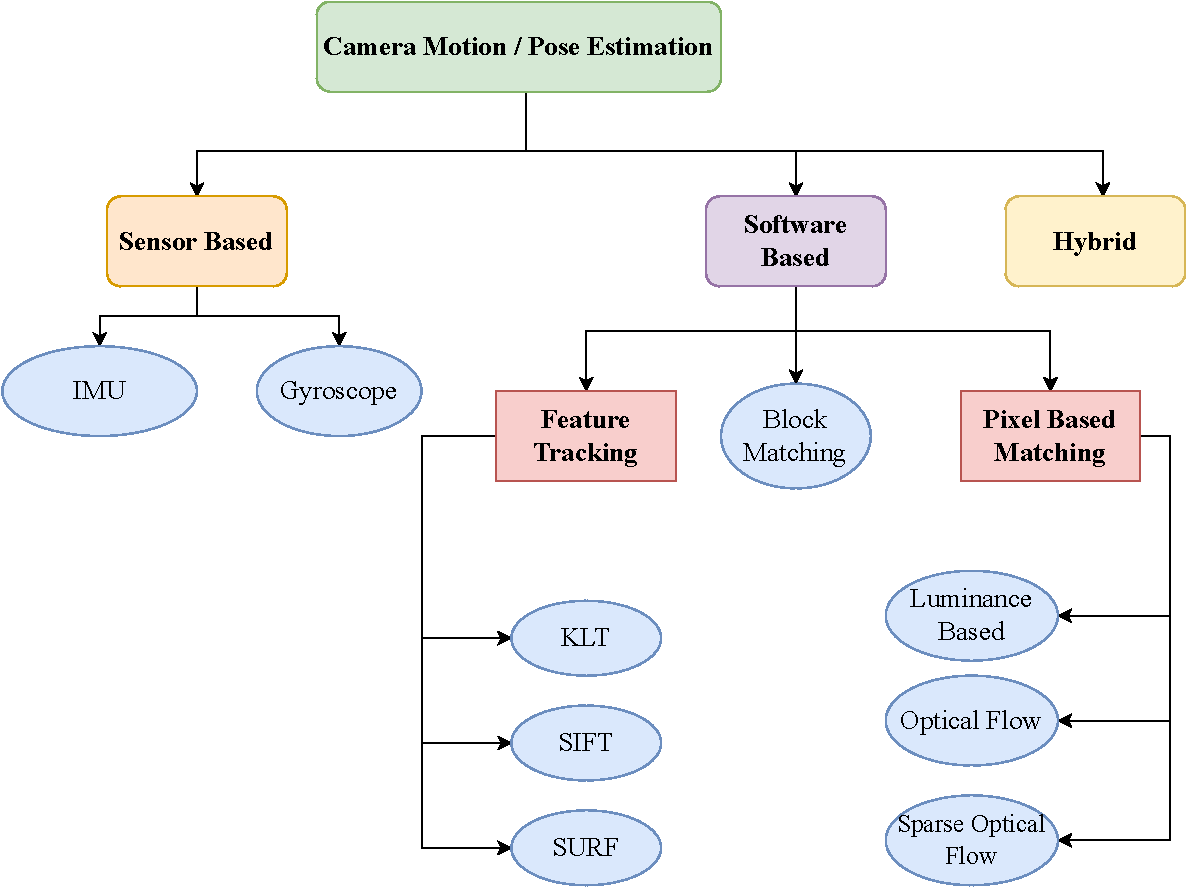
\includegraphics[scale=0.6]{images/fig_chapter2/cam_pose_estimation.pdf}
\caption{Camera Motion/Pose Estimation Techniques}
\label{fig:cam_pose_est}
\end{figure}

IMU sensors are widely used for pose estimation in image stabilization. I will go into depth about IMU sensors in the next section of this report. There are many other software based pose estimation techniques. 

\subsection{Software based motion estimation techniques}

Software based motion estimation techniques/algorithms use the images (frames) coming from the camera for motion estimation and subsequently for stabilization. Some of these software based techniques are listed below \citep{dis_review}:

\begin{itemize}
\item Pixel-based matching
\item Block-Matching
\item Feature-Matching
\end{itemize}

I will now briefly discuss how each of these approaches/algorithms are used in estimation of camera movements. This will also lay a foundation for the reasons as to why I am not using any of these techniques for my research.

\subsubsection{Pixel-Based Matching}
This method estimates pose by determining the motion of pixels between two frames \citep{dis_review}. For correspondence determination, luminance of two consecutive frames is assumed to be constant throughout. This poses a problem and there can be many pixels having same luminance, so, other constraints are also needed to obtain a unique solution \citep{dis_review}. 

Finding  \textbf{\textit{Optical Flow}} between two consecutive frame is another method for motion estimation. Optical flow is the distribution of apparent velocities of movement of brightness patterns in an image \citep{horn1981determining}. This gives us important information about the spatial arrangement of the objects viewed and the rate of change of this arrangement \citep{gibson1977analysis}. Using this information, relative motions can be estimated between consecutive image frames. These relative motions can be used for camera pose estimation. Many modern neural network based optical flow algorithms have also been developed recently and are used in image stabilization tasks \citep{deep_opti_stab}. Although this method can give us good results, but, it has very high computational requirements and thus can be very slow.

\subsubsection{Block-Matching}
Block matching techniques use blocks of pixels for motion estimation instead of finding correspondence between pixels of consecutive frames. This allows to remove some ambiguities that occur in pixel-based matching methods \citep{dis_review}. Block-matching approach offers a flexible trade-off between complexity, computational efficiency and accuracy \citep{dis_review}.

\subsubsection{Feature-Matching (Tracking)}
In these methods, the algorithm first selects the features that are easily recognisable and distinguishable. The motion is estimated by tracking only these features, so, this make them computationally less expensive. There are several feature tracking algorithms that are widely used in many computer vision applications.

\paragraph{}\textbf{Kanade Lucas Tomasi (KLT) feature tracker} \citep{tomasi1991detection} is a widely used feature tracking algorithm in computer vision. Features are selected and their position is initialized using this technique and then optical flow is used to track their position \citep{dis_review}.

\paragraph{}\textbf{Scale-invariant feature transform (SIFT)} is also used for motion estimation in digital image stabilization algorithms.  It has been designed for extracting highly distinctive invariant features from images, which can be used to perform reliable matching of the same object or scene between different images \citep{battiato2007sift}. It contains the orientation of the feature in order to be rotation-invariant \citep{dis_review}.

\paragraph{}\textbf{Speeded up robust features (SURF)} is inspired by SIFT but is faster \citep{dis_surf}. This technique is also widely used in feature selection and tracking for motion estimation.

I discussed about motion estimation from images and the common theme here is feature detection (be it a pixel, or a group of pixels or any other particular image feature) and then tracking it for motion estimation. But, there are certain use cases like mine where feature tracking is very difficult or unreliable. There are also situations where the features in an image are moving in different directions, which makes reliable motion estimation using these techniques impossible. This is the case for my research and my goal is to estimate pose which in invariant to what image is being captured. For this purpose I have decided to use sensor based pose-estimation techniques.

\subsection{Sensor based motion estimation techniques}
Pose estimation is a huge are of research especially for the field of robotics and autonomous driving. There are various sensors like Accelerometers, Gyroscopes, Magnetometers and Satellite Navigation systems available. For camera pose estimation, generally Gyroscopes and Accelerometers are used. In combination, these two sensors are called Inertial Measure Unit Sensors. I will talk in depth about how these sensors are use for pose estimation in the next section of this report. For my research I will use this sensor for pose estimation as using it has many advantages. And it's use will make my stabilization algorithm image invariant which is highly desirable for my use case.

% Start: IMU Sensors
\section{Inertial Measurement Unit (IMU) Sensors}
IMU sensor is one of the most commonly used sensors in the world and present all around us in mobile devices, Virtual Reality gear and camera. It is very common to use IMU sensor for pose estimation. An IMU sensor measures acceleration(m/s²) and angular velocity (rad/s).  They can make these measurements in multiple degrees of freedom. For example, a 6-DoF IMU sensor includes a 3-axis accelerometer and 3 axis gyroscope  \citep{constant2021data}. The accelerometer will make independent acceleration measurements in let's say x, y and z directions. Similarly the gyroscope makes independent angular velocity measurements about these three axis.

IMU sensors are used in a wide variety of applications like navigation, robotics, drones, smart watches, sports learning, augmented reality systems, industrial quality control \citep{ahmad2013reviews}  and also for image stabilization in cameras. In all these applications, IMU sensor is used for pose estimation in some form; either for absolute pose estimation or change in pose. It is important to note that for my application here the IMU will be strapped on to the camera system. Which means the IMU sensor can has all 6 of its DoF.

There are a lot of reasons to use IMU sensors and these reasons are surely a very huge contributor to them being one of the most commonly used sensors in the world. Some of their qualities are \citep{woodman2007introduction}.:

\begin{itemize}
\item They have small size, 
\item low weight, 
\item rugged construction, 
\item low power consumption, 
\item cheap, 
\item high reliability, 
\item low maintenance
\item can be used in hostile environments 
\end{itemize}

\subsection{Pose Estimation with IMUs}
Pose for any object is its position(x, y, z) and its orientation(yaw, pitch, roll) with respect to some reference coordinate system. To calculate pose of an object, we continuously take measurements from IMU and using some algorithms we calculate the pose. Figure \ref{fig:strapdown_imu} below shows the strap-down inertial navigation algorithm \citep{woodman2007introduction}.

\begin{figure}
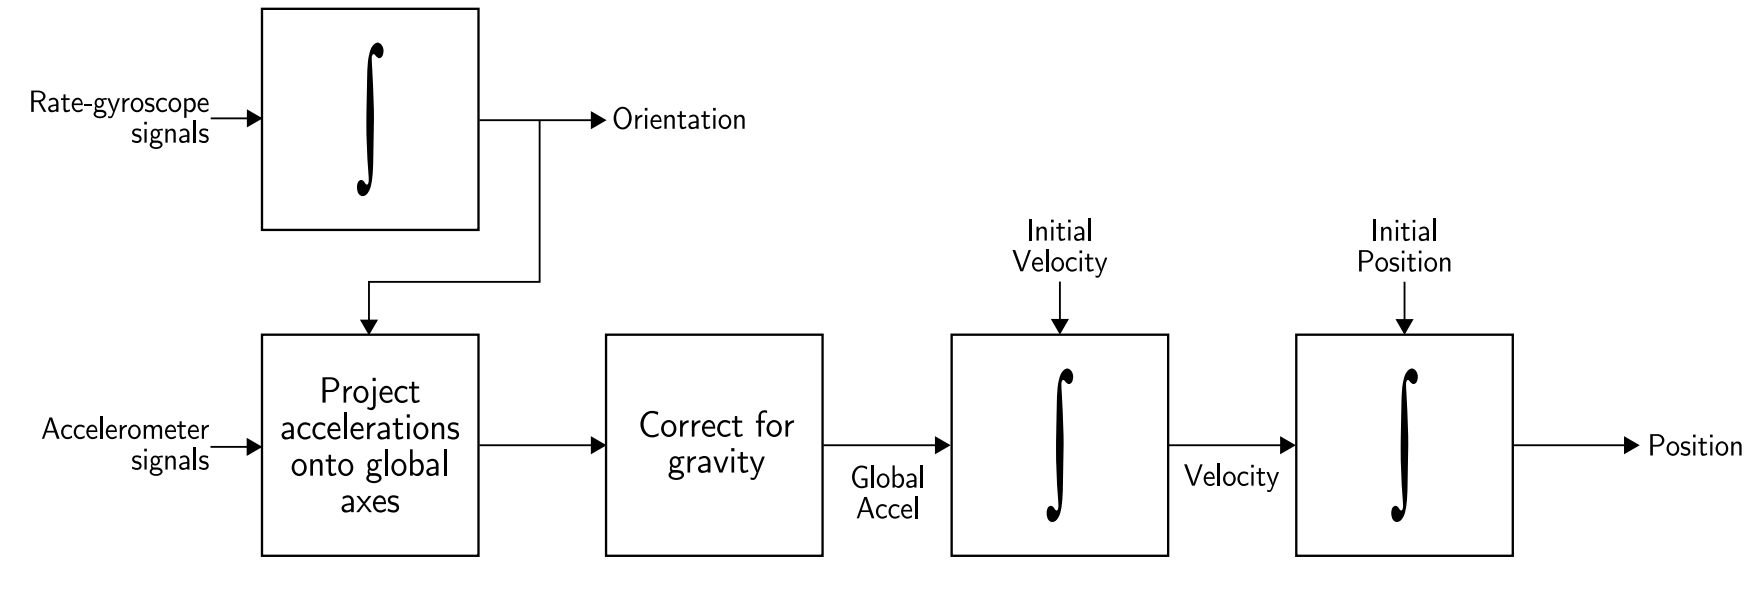
\includegraphics[scale=0.2]{images/fig_chapter2/strap_imu_algo.png}
\caption{Strap-down inertial navigation algorithm \citep{woodman2007introduction}}
\label{fig:strapdown_imu}
\end{figure}

Based on the algorithm we can see that to estimate the pose, we need to do integration on Gyroscope values to get orientation. And double integration on Accelerometer values to get the position. That seems simple but the IMU readings are not ideal, they contain noises and biases \citep{woodman2007introduction} which need to be accounted for.

\subsection{IMU Noise Models}
Sensor outputs are inherent to noise. There is different types of noise with which we have to deal. For IMUs, the readings coming from a sensor could be modelled as a combination of three entities: pure signal, bias and white noise.

\textbf{Gyroscope}
\begin{equation}
    \omega_{n}(t) = \omega(t) + b_{g}(t) + n_{g}
\label{eqn:gyro_noise}
\end{equation}

Where $ \omega_{n}(t) $ is the noisy gyroscope signal, $ \omega(t) $ is the pure gyroscope signal, $ b_{g}(t) $ is the gyroscope bias and $ n_{g} $ is the gyroscope white noise.

\textbf{Accelerometer}
\begin{equation}
    a_{n}(t) = a(t) + b_{a}(t) + n_{a}
\label{eqn:accel_noise}
\end{equation}

Where $ a_{n}(t) $ is the noisy accelerometer signal, $ a(t) $ is the pure accelerometer signal, $ b_{a}(t) $ is the accelerometer bias and $ n_{a} $ is the accelerometer white noise.

For both gyroscope and accelerometer the signal can be independently modeled this way in each of its axis (x, y and z) \citep{imu_noise}. Although the modelling equation looks the same for both IMU and but they have different effects on pose estimation as the strap-down inertial algorithm suggests.

To demonstrate the \textit{Noise Model}, let's take a pure unit signal as show in figure \ref{fig:imu_noise} a. \textbf{Bias} can be defined as a noise in signal which is linearly increasing with time as show in figure \ref{fig:imu_noise} (Note: Bias can be subtractive too, here it is shown as additive and the bias in the figure is an exaggeration for demonstration purpose). If we add the bias to the pure signal it will look something like as show in figure \ref{fig:imu_noise} b (right). Another component to the noisy signal is white noise. This can be modeled as random data with zero mean ($ \mu = 0 $) and some variance ($ \sigma^{2} $) and is shown in figure \ref{fig:imu_noise} b (right). Based on equations \ref{eqn:gyro_noise} and \ref{eqn:accel_noise} the bias and white noise will be added to the signal and it will look like as show in figure \ref{fig:imu_noise} c (right). 

\begin{figure}
  \begin{subfigure}{\linewidth}
  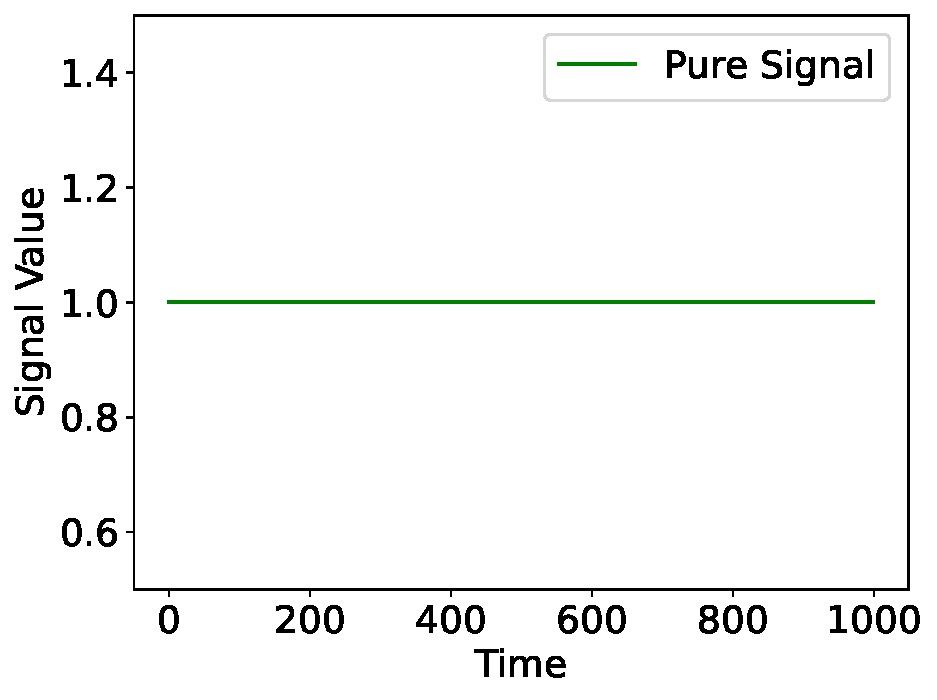
\includegraphics[width=.55\linewidth]{images/fig_chapter2/noise_figs/pure_signal.pdf}\hfill
  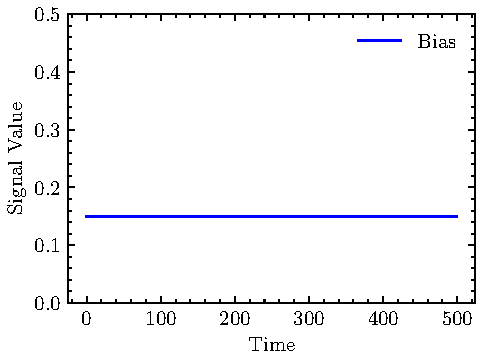
\includegraphics[width=.55\linewidth]{images/fig_chapter2/noise_figs/bias.pdf}
  \caption{Pure Signal and bias}
  \end{subfigure}\par\medskip
  \begin{subfigure}{\linewidth}
  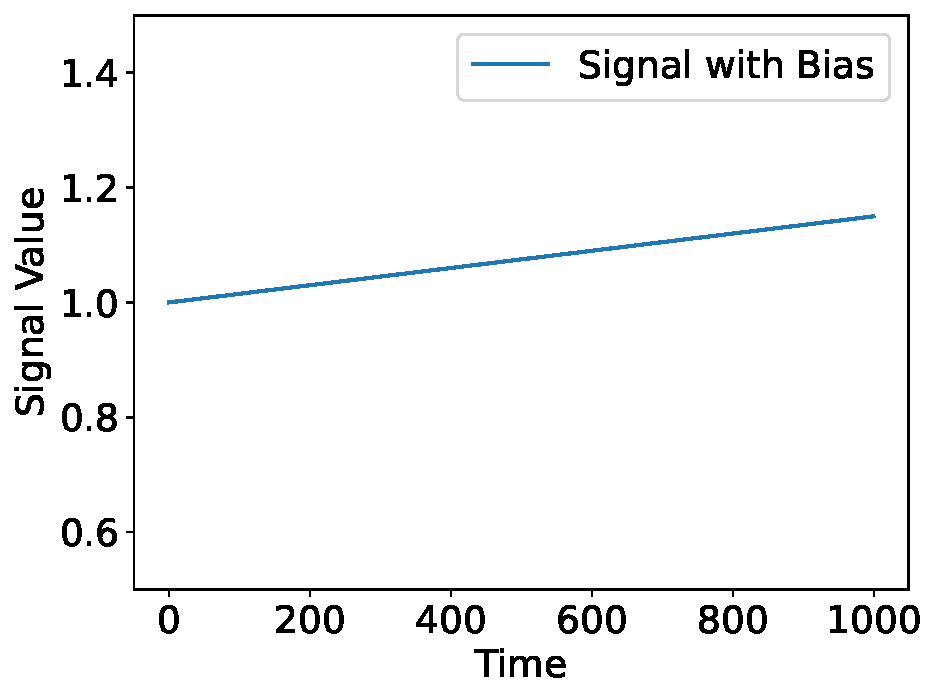
\includegraphics[width=.55\linewidth]{images/fig_chapter2/noise_figs/signal_bias.pdf}\hfill
  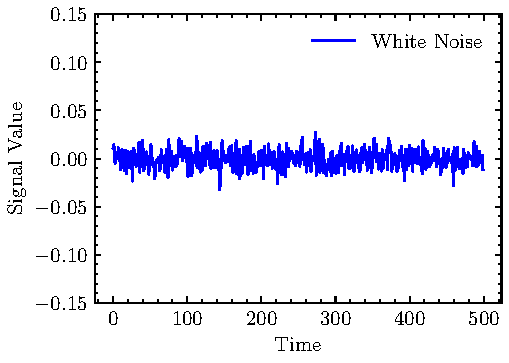
\includegraphics[width=.55\linewidth]{images/fig_chapter2/noise_figs/white_noise.pdf}
  \caption{Signal with bias and white noise}
  \end{subfigure}\par\medskip
  \begin{subfigure}{\linewidth}
  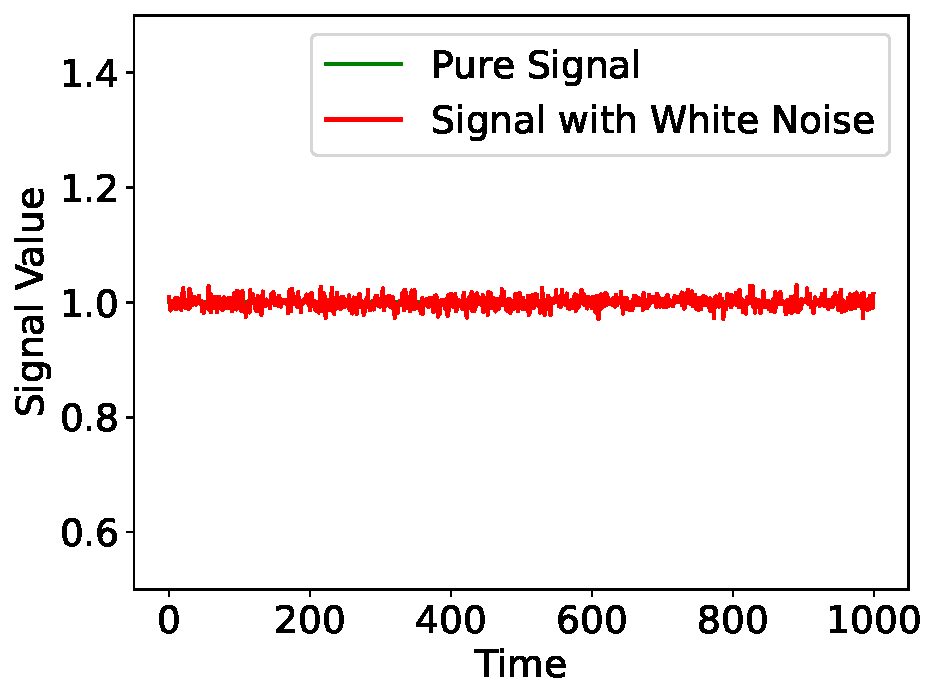
\includegraphics[width=.55\linewidth]{images/fig_chapter2/noise_figs/signal_white_noise.pdf}\hfill
  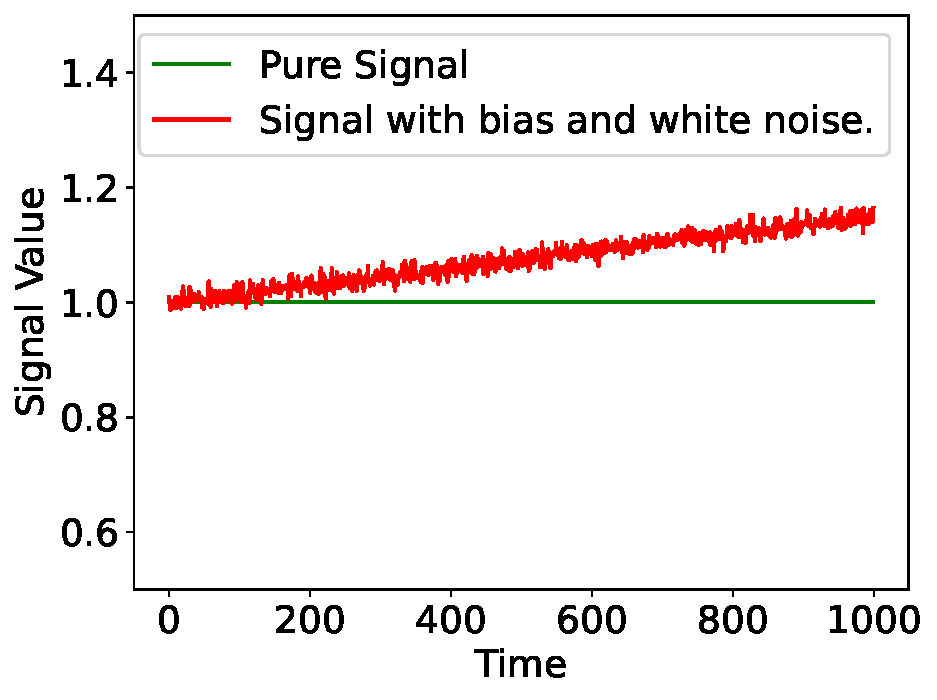
\includegraphics[width=.55\linewidth]{images/fig_chapter2/noise_figs/signal_white_noise_bias.pdf}
  \caption{Signal with white noise and signal with white noise and bias}
  \end{subfigure}
  \caption{Noise Model Demonstration}
\label{fig:imu_noise}
\end{figure}

As you can see from the plots, the noisy signal looks very different from the pure signal. Using the noisy signal directly for pose estimation can lead to very inaccurate results. There are various signal processing techniques/algorithms which can be used to mitigate this issue and will be discussed in the upcoming sections of this report.

\subsubsection{Gyro Error Characteristics}
To get orientation from the gyroscope, the readings need to be integrated once and the global orientation needs to be updated. This needs to be done for each of the gyroscope axis. Doing this continuously with the noisy signal will result into erroneous  orientation tracking if nothing is done about the noise. In table \ref{tab:gyro_error} you can see all the errors and effect of those on orientation measurement.

% gyro error table
\begin{table}[ht]
    \centering
\begin{tabular}{ l| L| L } \hline
     \thead{Error Type} & \thead{Description} & \thead{Result of Integration} \\ \hline
     Bias & 
     A constant Bias epsilon & 
     Steadily growing angular error.  \[\theta(t) = \epsilon.(t)\] \\
     \hline
     White Noise & 
     White noise with some standard deviation sigma & 
     An angular random walk, whose standard deviation grows with the square root of time. 
     \[\sigma_\theta(t) = \sigma.\sqrt{\delta.t}\] \\
     \hline
     Temperature Effects & 
     Temperature dependent residual bias & 
     Any residual bias is integrated into orientation, causing an orientation error which grows linearly with time. \\
     \hline
     Calibration & 
     Deterministic errors in scale factors, alignments and gyro linearities & 
     Orientation drift proportional to the rate and duration of motion. \\
     \hline
     Bias Instability & 
     Bias fluctuations, usually modelled as a bias random walk & 
     A second order random walk. \\
     \hline
\end{tabular}
    \caption{Summary of Gyro Error Sources \citep{woodman2007introduction}}
    \label{tab:gyro_error}
\end{table}

\subsubsection{Accelerometer Error Characteristics}
Generating position information from accelerometer is not a single step like in case of Gyroscope. As you can see in the strap-down inertial navigation algorithm shown in figure \ref{fig:strapdown_imu} there are multiple steps involved. First, the accelerometer readings need to projected into the global axis using the orientation calculated from gyroscope. Then, the accelerometer reading needs to be corrected for gravity. After that we double integrate the signal based on initial velocity and initial position to finally get the position.

So, there is double integration present in the algorithm. We also have a noisy signal, so, the noise also gets integrated two times. This can result into very inaccurate position estimations and is one of the most challenging parts of working with an IMU. In table \ref{tab:accel_error} you can see all errors in an MEMS accelerometer and effect of those on position measurement.

% accelerometer error table
\begin{table}[ht]
    \centering
\begin{tabular}{ l| L| L } \hline
     \thead{Error Type} & \thead{Description} & \thead{Result of Double Integration} \\ \hline
     Bias & 
     A constant Bias epsilon in the accelerometer's output signal. & 
     A quadratically growing position error. \[s(t) = \epsilon . \frac{t^{2}}{2}\]   \\
     \hline
     White Noise & 
     White noise with some standard deviation sigma & 
     A second order random walk. The standard deviation of the position error grows as
     \[\sigma_s(t) = \sigma . t^{\frac{3}{2}} . \sqrt{\frac{\sigma . t}{3}}\]   \\
     \hline
     Temperature Effects & 
     Temperature dependent residual bias & 
     Any residual bias causes an error in position which grows quadratically with time. \\
     \hline
     Calibration & 
     Deterministic errors in scale factors, alignments and accelerometer linearities & 
     Position drift proportional to the squared rate and duration of acceleration. \\
     \hline
     Bias Instability & 
     Bias fluctuations, usually modelled as a bias random walk & 
     A third-order random walk in position. \\
     \hline
\end{tabular}
    \caption{Summary of Accelerometer Error Sources \citep{woodman2007introduction}}
    \label{tab:accel_error}
\end{table}

\subsubsection{Challenges in Working with IMU}
As you can see it is not straightforward to work with IMUs, especially for absolute position estimation as the errors introduced are squared with time. This results in a \textbf{drift} from actual position, which for any image stabilization algorithm is very detrimental. Orientation estimation is still relatively reliable and is the main reason why Gyroscope based hardware as well as digital image stabilization is more common. 

These issues presents a lot of challenges especially for our case, as we require a precision in the range 0.1 mm. So, the sensor readings cannot be used directly in the inertial navigation algorithm. Generally some basic (Low pass, moving average filter) and advanced signal processing techniques and algorithms like Madgwick, Kalman Filter and its other versions are used to estimate the pose using IMU. These techniques may be good enough for some other applications, but in our case their use is not enough. The precision requirements are very high. Even with the use of these algorithms, there is still a drift present which is unacceptable for this use case. In the next section I will discuss about pose estimation using IMU sensors.

% Start: Pose Estimation
\section{Pose Estimation using IMU}
There are classical and modern approaches that I will discuss in this section.

\subsection{Classical Algorithms}
\subsubsection{Signal Filtering}
\begin{itemize}
\item Low pass
\item Moving Average
\item Kalman filter
\item Madgwick Filter
\end{itemize}

\subsection{Neural Network Based}
Using Neural networks for pose estimation
\begin{itemize}
\item RIDI
\item RoNIN
\item CTIN
\end{itemize}